\documentclass[tikz,border=10pt]{standalone}
\usetikzlibrary{shapes.geometric,backgrounds,calc}
\tikzset{
  basic box/.style = {
    shape = rectangle,
    align = center,
    draw  = #1,
    fill  = #1!25,
    minimum width = 3cm,
    minimum height = 0.8cm,
    rounded corners}
}
\begin{document}
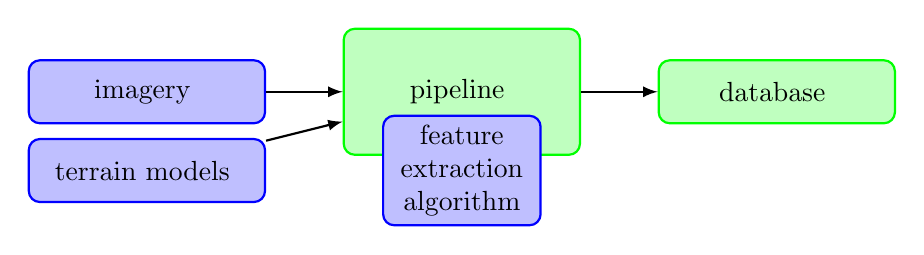
\begin{tikzpicture}[node distance = 4cm, thick, nodes = {align = center}, >=latex]
  \node[basic box = blue, anchor = west, yshift = -1cm] (terrain) { terrain models };
  \node[basic box = blue, anchor = west] (imagery) { imagery };
  \node[basic box = green, anchor = center, right of = imagery, minimum height = 1.6cm] (pipeline) { pipeline };
  \node[basic box = green, anchor = east, right of = pipeline] (database) { database };
  \node[basic box = blue, below of = pipeline, yshift=3cm, minimum width = 2cm](alg) {feature \\ extraction \\ algorithm};
  \draw[->]    (imagery) -- (pipeline);
  \draw[->]    (terrain) -- (pipeline);
  \draw[->]    (pipeline) -- (database);
\end{tikzpicture}
\end{document}
